%        File: main.tex
%     Created: Tue Jan 17 11:00 AM 2017 E
% Last Change: Tue Jan 17 11:00 AM 2017 E
%

\documentclass{beamer}
\usetheme{Frankfurt}
\usepackage{common}

  \title{Aerothermodynamic Design Sensitivities for a Reacting Gas Flow Solver
  on an Unstructured Mesh Using a Discrete Adjoint Formulation}

  \author{ Kyle B. Thompson }
  \institute[North Carolina State University and NASA Langley Research Center]{
    Mechanical and Aerospace Engineering Department \\
    North Carolina State University
    \and
    Aerothermodynamics Branch \\
    NASA Langley Research Center}

% Date of the Oral Preliminary Exam
\date{Month Day, 2017}

% This turns off the navigation bar at the bottom of each frame
\beamertemplatenavigationsymbolsempty

\begin{document}
\setbeamertemplate{caption}{\raggedright\centering\insertcaption\par}
\begin{frame}
  \titlepage
\end{frame}
\begin{frame}
  \frametitle{Outline}
  \tableofcontents
\end{frame}
\section{Introduction}
\stepcounter{subsection}
\begin{frame}
  \frametitle{Introduction - Design}
  \begin{itemize}
    \item Gradient-based design optimization is based on the minimization of a target
      ``cost'' function by changing a set of design variables
    \item A CFD code can be coupled with a numerical optimization package to
      iteratively improve target aerothermodynamic quantities, by change inputs to
      the CFD code
  \end{itemize}
  \begin{figure}[h]
    \centering
    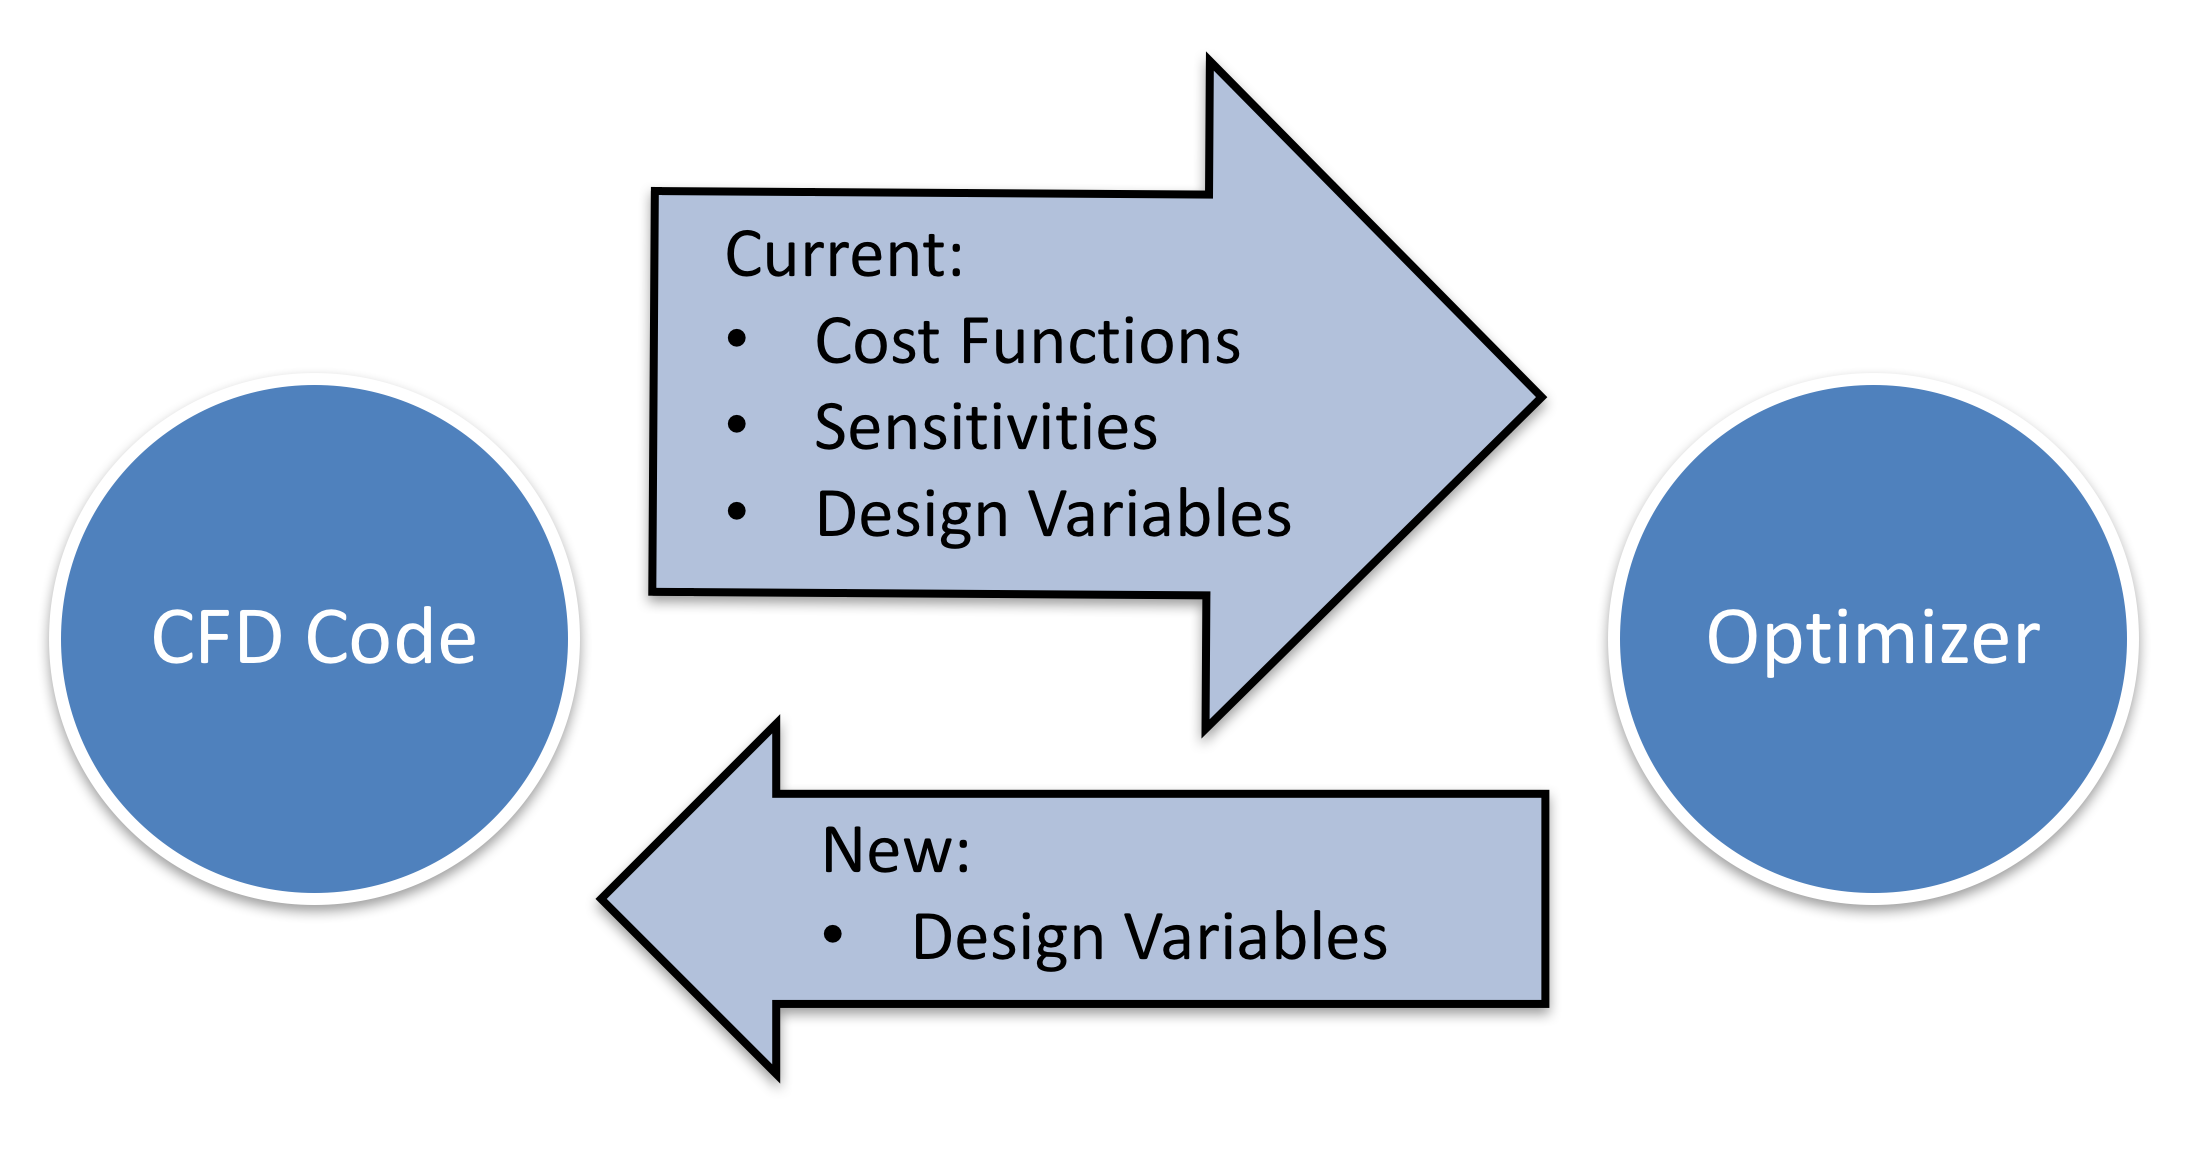
\includegraphics[width=0.6\textwidth]{figures/cfd-optimizer.png}
    \caption{CFD-Optimizer Relationship}
    \label{fig:cfd-opt}
  \end{figure}
\end{frame}
\begin{frame}
  \frametitle{Introduction - Design}
  \begin{itemize}
    \item The top-level design process is simple, but CFD sensitivity analysis 
      is expensive
    \item<2-> Need efficient way to compute cost function sensitivities for
      large number of design variables
  \end{itemize}
  \only<3>{\begin{tcolorbox}[colback=red!5!white,colframe=red!75!black, 
    title = Direct differentiation approach - Expensive]
    \begin{itemize}
      \item Navier-Stokes equations can be directly differentiated to yield
        sensitivity derivatives necessary for gradient-based optimization
      \item Finite difference requires a minimum of \textbf{one flow solution
        for each design variable sensitivity}
      \item Prohibitively expensive for large number of design variables
    \end{itemize}
  \end{tcolorbox}}
  \only<4>{\begin{tcolorbox}[colback=green!5!white,colframe=green!75!black,
    title = Adjoint approach - More efficient]
    \begin{itemize}
      \item Solve adjoint equations in addition to Navier Stokes flow equations to
        obtain sensitivity derivatives
      \item \textbf{One flow and adjoint solution needed for each cost function},
      regardless of number of design variables
      \item Considerably more efficient than direct differentiation approach for
        large number of design variables
    \end{itemize}
  \end{tcolorbox}}
\end{frame}
\begin{frame}
  \frametitle{Introduction - Design}
  \begin{itemize}
    \item Adjoint-based design optimization is widely adopted in compressible,
      perfect gas CFD solvers
    \item Reacting flow solvers have lagged in adopting adjoint-based approach,
      due to
    \begin{enumerate}
      \item Complexity of linearizing the additional equations for
        multi-species chemical kinetics
      \item Resorting to Automatic Differentiation tools incurs performance
        overhead that is implementation-specific
      \item Serious memory and computational cost concerns when simulating a
        large number of species
    \end{enumerate}
    \item Points 1 and 2 can be overcome through stubbornness (or hiring a
      graduate student\dots)
    \item Point 3 is a serious concern, if reacting flow solver are to be made
      attractive for design optimization
  \end{itemize}
\end{frame}
\begin{frame}
  \frametitle{Introduction - Improvement to State of the Art}
  \begin{itemize}
    \item Current state of the art
      \begin{itemize}
        \item Attempts made at both continuous\fcite{Copeland} and
          discrete\fcite{Lockwood} adjoint formulations
          for a compressible reacting flow solver
        \item These attempts suffer from quadratic scaling in memory and
          computational cost with number of species
        \item Recent scheme at Barcelona Supercomputing
          Center\fcite{Esfahani:2016aa} is promising, but only for
          incompressible reacting flows
      \end{itemize}
    \item Improvement to the state of the art
      \begin{itemize}
        \item New decoupled scheme for both hypersonic flow solver and adjoint
          solver that is robust for high-speed flows in chemical non-equilibrium
        \item New schemes significantly improve scaling in computational cost
          and memory with number of species
      \end{itemize}
  \end{itemize}
\end{frame}
\begin{frame}
  \frametitle{Introduction - Decoupled Approach}
  \begin{itemize}
    \item Reacting gas simulations require solving a large number of conservation
      equations
    \item Memory concerns
    \begin{itemize}
        \item Size of Jacobians scales quadratically with number species in gas mixture
        \item Solving system of equations in a tightly-coupled fashion can be
          limited by memory constraints
    \end{itemize}
    \item Cost concerns
    \begin{itemize}
      \item Cost of solving the linear system scales quadratically with number
      of species in gas mixture
    \end{itemize}
    \item Efficiently solving adjoint problem is a primary motivator
      \begin{itemize}
        \item Solving adjoint system particularly costly if linear solver is
          slow
        \item Can be necessary to store jacobian twice $\to$ large memory
          overhead
      \end{itemize}
  \end{itemize}
\end{frame}
\begin{frame}
  \frametitle{Introduction - Decoupled Approach}
  \begin{itemize}
    \item Loosely-coupled solvers have become popular in the combustion
      community\fcite{Sankaran}
      \begin{itemize}
        \item Decouple species conservation equations from meanflow equations,
          and solve two smaller systems
         \[
           \underset{(4+ns) \times (4+ns)}
           {\begin{pmatrix}
             \boxempty & \boxempty & \dots  & \boxempty \\
             \boxempty & \boxempty & \dots  & \vdots \\
             \vdots    & \vdots    & \ddots & \vdots \\
             \boxempty & \dots     & \dots  & \boxempty
           \end{pmatrix}}
           \to
           \underset{5 \times 5}
           {\begin{pmatrix}
             \boxempty & \dots  & \boxempty \\
             \vdots    & \ddots & \vdots \\
             \boxempty & \dots  & \boxempty
           \end{pmatrix}}
           \text{and}
           \underset{ns \times ns}
           {\begin{pmatrix}
             \boxempty  & \boxbslash & \dots  & \boxbslash \\
             \boxbslash & \boxempty  & \dots  & \vdots \\
             \vdots     & \vdots     & \ddots & \vdots \\
             \boxbslash & \dots      & \dots  & \boxempty
           \end{pmatrix}}
         \]
    \end{itemize}
  \item Candler, et al.\fcite{candler} originally derived this for
    Steger-Warming scheme, this work extends to Roe FDS scheme
  \end{itemize}
\end{frame}

\AtBeginSection[]
{
 \begin{frame}<beamer>
 \frametitle{Outline}
 \tableofcontents[currentsection]
 \end{frame}
}
\section{Flow Solver}

\subsection{Fully-Coupled Flow Solver}
\stepcounter{subsection}
\begin{frame}
  \frametitle{Fully-Coupled Point Implicit Flow Solver}
  \begin{itemize}
    \item All work presented is for inviscid flows in chemical non-equilibrium,
      using a one-temperature model, but is extendable to viscous flows.
    \item Beginning with the semi-discrete form
    \begin{equation*}
    	\label{inv_flux_fv}
    	\frac{\partial \mU}{\partial t}
    	 + \frac{1}{V}\sum\limits_{f}(\vF\cdot\ms)^f = \mw
    \end{equation*}
    \begin{equation*}
    	\begin{matrix}
    	\mU=\begin{pmatrix}
       		\rho_1\\
    		\vdots \\
    		\rho_{ns} \\
    		\rho u \\
    		\rho v \\
    		\rho w \\
    		\rho E \\
    	\end{pmatrix},      &
     	\mathbf{F \cdot S} = \begin{pmatrix}
    		\rho_1  \overline{U} \\
    		\vdots \\
    		\rho_{ns} \overline{U} \\
    		\rho u \overline{U} + p s_x\\
    		\rho u \overline{U} + p s_y\\
    		\rho u \overline{U} + p s_z\\
    		(\rho E + p) \overline{U} \\
    	\end{pmatrix}S,    &
     	\mw = \begin{pmatrix}
        \dot\rho_1\\
    		\vdots \\
    		\dot\rho_{ns} \\
        0 \\
        0 \\
        0 \\
        0
      \end{pmatrix}

  	\end{matrix}
  \end{equation*}

  \end{itemize}
\end{frame}
\begin{frame}
  \frametitle{Fully-Coupled Point Implicit Flow Solver}
  \begin{itemize}
  \item Using the Roe FDS scheme to compute the inviscid flux at the face,
    $\vF^f$, and linearizing the system results in
  \begin{multline*}
  	\frac{\mathbf{\delta U}^n}{\Delta t}
    +\frac{1}{V}\sum\limits_{f}(\frac{\partial \vF^f}
    {\partial \ul}\delta\mU^L
  	+\frac{\partial \vF^f}{\partial \ur}\delta\mU^R)^n \ms^f
  	- \frac{\partial \mw}{\partial \mU}\delta\mU^n \\
  	= -\frac{1}{V}\sum\limits_{f}(\vF^f\cdot\ms^f)^n + \mw^n
  \end {multline*}
  \item Which can be thought of more simply as
  \[
    \ma\vu = \vb
  \]
  \vspace{-0.7cm}
  \begin{align*}
    \ma &\to
    \begin{array}{c}
      (4+ns) \times (4+ns) \\
      \text{Jacobian Block}
    \end{array} \\
    \vb &\to
    \begin{array}{c}
      (4+ns) \times 1 \\
      \text{Residual}
    \end{array}
  \end{align*}
  \end{itemize}
\end{frame}
\begin{frame}
  \frametitle{Fully-Coupled Point Implicit Flow Solver}
  \begin{itemize}
    \item Constructing the Jacobian in a fully-coupled fashion results in large,
      dense block matricies
    \item Using a stationary iterative method (i.e., Gauss-Seidel, SSOR, etc.),
      work is dominated by matrix-vector products
      \[
        \text{Cost} \to O((4+ns)^2)
      \]
    \item Leads to onerous quadratic scaling with respect to number of species
  \end{itemize}
\end{frame}

\subsection{Decoupled Flow Solver}
\stepcounter{subsection}

\begin{frame}
  \frametitle{Decoupled Point Implicit Flow Solver}
  \begin{itemize}
    \item The main idea is to separate the meanflow and species composition
      equations, adding a new equation for the total mixture density
    \item Leads to two sets of conserved variables
      \begin{equation*}
      	\begin{matrix}
      		\mU'=\begin{pmatrix}
      			\rho \\
      			\rho u \\
      			\rho v \\
      			\rho w \\
      			\rho E
      		\end{pmatrix} &
      		\mathbf{\hat{U}}=\begin{pmatrix}
      			\rho_1 \\
      			\vdots \\
      			\rho_{ns}
      		\end{pmatrix} \\ \\
          \text{Meanflow} & \text{Species Composition}
      	\end{matrix} 
      \end{equation*}
  \end{itemize}
\end{frame}

\begin{frame}
  \frametitle{Decoupled Point Implicit Flow Solver}
  \begin{itemize}
    \item The fluxes are solved in two sequential steps
      \begin{itemize}
        \item  The mixture fluxes are first solved as
        \[
          \frac{\partial \mU'}{\partial t} +
          \frac{1}{V}\sum\limits_{f}(\vF'\cdot\ms)^f = 0
        \]
      \item Followed by the species fluxes
      \[
        \frac{\partial \mathbf{\hat{U}}}{\partial t} +
        \frac{1}{V}\sum\limits_{f}(\mathbf{\hat{F}}\cdot \ms)^f =
        \mathbf{\hat{W}}
      \]
    \end{itemize}
    \item Since the mixture density was determined in the first step, step two
      actually solves for the species mass fractions
      \begin{gather*}
        \delta \mathbf{\hat{U}}^n 
        = \rho^{n+1} \hat{\mv}^{n+1}-\rho^n\mathbf{\hat{V}}^n = \rho^{n+1} \delta
        \mathbf{\hat{V}}^n + \mathbf{\hat{V}}^n \delta \rho^n \\
        \mathbf{\hat{V}}=(c_1,\hdots,c_{ns})^T, c_s=\rho_s/\rho
      \end{gather*}
  \end{itemize}
\end{frame}
\begin{frame}
  \frametitle{Decoupled Point Implicit Flow Solver}
  \begin{itemize}
    \item The Roe FDS scheme species mass fluxes can be rewritten as
      \begin{align*}
  	\hat{\vF}_{\rho_s} &= c_s \vF'_\rho+(c_s^L-\tilde{c}_s)\rho^L\lambda^+
  	+ (c_s^R-\tilde{c}_s)\rho^R\lambda^- \\
	\frac{\partial \hat{\vF}_{\rho_s}}{\partial c_s^L} 
	&= w\vF_\rho+(1-w)\rho^L\lambda^+ - w\rho^R\lambda^- \\
	\frac{\partial \hat{\vF}_{\rho_s}}{\partial c_s^R} 
	&= (1-w)\vF_\rho+(w-1)\rho^L\lambda^+ + w\rho^R\lambda^- \label{d_last}
      \end{align*}
    \item Jacobian Approximations
      \begin{align*}
	\text{Step 1:}\quad &
	\frac{\partial \vF}{\partial \mU'}\bigg|_{\mathbf{\hat{V}}} =
	\underset{c_s = \text{Constant}}{5 \times 5\,\text{Roe FDS Jacobian}} \\
	\text{Step 2:}\quad & 
	\frac{\partial \vF}{\partial \hat{\mv}}\bigg|_{\mathbf{\hat{U'}}} = 
        \begin{pmatrix} 
          \frac{\partial F_{\rho_1}}{\partial c_1} & & 0
          \\ & \ddots &  \\ 0 & & \frac{\partial F_{\rho_{ns}}}{\partial c_{ns}}
        \end{pmatrix} 
      \end{align*}
  \end{itemize}
\end{frame}
\begin{frame}
  \frametitle{Decoupled Point Implicit Flow Solver}
  \vspace{-0.2cm}
  \begin{itemize}
    \item Chemical source term linearized via
    \vspace{-0.1cm}
    \begin{align*}
      \mathbf{\hat{W}}^{n+1} &= \mathbf{\hat{W}}^n+\frac{\partial
      \mathbf{\hat{W}}}{\partial \mathbf{U}}\bigg|_{\mathbf{U}'} \frac{\partial
      \mathbf{U}}{\partial \mathbf{\hat{V}}} \\
       \mc &= \frac{\partial \mathbf{\hat{W}}}{\partial
       \mathbf{U}}\bigg|_{\mathbf{U}'} \frac{\partial \mathbf{U}}{\partial
       \mathbf{\hat{V}}}
    \end{align*}
    \item Full system to be solved in step two
    \vspace{-0.2cm}
    \begin{gather*}
      \begin{split} \rho^{n+1}&\frac{\delta \hat{\mv}^n}{\Delta t}
        +\frac{1}{V}\sum\limits_{f}(\frac{\partial \hat{\vF}^f}{\partial
        \mv^L}\delta \mv^L +\frac{\partial
        \hat{\vF}^f}{\partial \hat{\mv}^R}\delta
        \hat{\mv}^R)^{n, n+1}\ms^f - \mc^{n, n+1}\delta\mv^n \\ &=
        -\frac{1}{V}\sum\limits_{f}(\hat{\vF}^{n,n+1}\cdot\ms)^f +
        \mw^{n, n+1} -\hat{\mv}^n\left(\frac{\delta \rho^n}{\Delta t} -
        R_\rho\right)
      \end{split} \\ 
    \end{gather*}
    \vspace{-1.4cm}
    \[
      R_\rho = -\frac{1}{V}\sum\limits_{f}{\sum\limits_{s}
      {(\hat{F}_{\rho_s}^{n,n+1}\cdot\mathbf{S})}}
    \]
  \item $R_\rho$ is included to preserve $\sum\limits_{s}{c_s}=1$, $\sum\limits_{s}{\delta c_s}=0$.
  \end{itemize}
\end{frame}

\subsection{Cost and Memory Savings of the Decoupled Flow Solver}

\begin{frame}
  \frametitle{Cost and Memory Savings of the Decoupled Flow Solver}
\begin{itemize}
  \item Most significant savings comes from the source term linearization being purely node-based
    \begin{itemize}
      \item Convective contributions to block Jacobians are diagonal
      \item Source term jacobian is dense block Jacobian
      \item In the global system (w/chemistry), all off-diagonal block jacobians
        are diagonal
    \end{itemize}
  \end{itemize}
  \[
    \begin{pmatrix} 
      \Box & & & & \\ 
      & \ddots & & & \\ 
      & & \Box \\ 
      & & & \ddots & \\ 
      & & & & \Box
    \end{pmatrix} \begin{pmatrix} \delta \mathbf{\hat{V}}_1 \\ \vdots \\ \delta
      \mathbf{\hat{V}}_i \\ \vdots \\ \delta \mathbf{\hat{V}}_{nodes}
    \end{pmatrix} = \begin{pmatrix} \hat{b}_1 \\ \vdots \\ \hat{b}_i \\ \vdots \\
      \hat{b}_{nodes} \end{pmatrix} - \begin{pmatrix}
      (\sum_{j=1}^{N_{nb}}{[\diagdown] \delta\mathbf{\hat{V}}_{j}})_1 \\ \vdots \\
      (\sum_{j=1}^{N_{nb}}{[\diagdown] \delta\mathbf{\hat{V}}_{j}})_i \\ \vdots \\
      (\sum_{j=1}^{N_{nb}}{[\diagdown] \delta\mathbf{\hat{V}}_{j}})_{nodes}
    \end{pmatrix} 
  \]
  \begin{itemize}
    \item Matrix-vector products $\to$ inner products: $O(ns^2) \to O(ns)$
  \end{itemize}
\end{frame}
\begin{frame}
  \frametitle{Cost and Memory Savings of the Decoupled Flow Solver}
  \begin{itemize}
    \item Comparing size of Jacobian systems, using Compressed Row Storage
  \end{itemize}
  \begin{align*}
    \ma_d &= \text{Decoupled system Jacobians} \\
    \ma &= \text{Fully-coupled system Jacobians}
  \end{align*}
  \[
  \begin{split} Relative\ Memory\ Cost &=
    \frac{size(\ma_d)}{size(\ma)} \\ &= \lim_{ns\to\infty}
    \frac{(ns^2+5^2)(N_{nodes})+(ns+5^2)(N_{nbrs})}{(ns+4)^2(N_{nodes}+N_{nbrs})} \\
    &= \frac{N_{nodes}}{N_{nodes} + N_{nbrs}}
  \end{split}
  \]
\end{frame}


\section{Adjoint Solver}
\stepcounter{subsection}
\subsection{Derivation of Discrete Adjoint Formulation}
\begin{frame}
  \frametitle{Derivation of Discrete Adjoint Formulation}
  \begin{itemize}
    \item The derivation of the adjoint approach to compute design sensitivities
      begins with forming the Lagrangian and differentiating with respect to the
      design variables
      \begin{gather*}
        L(\md,\mq,\mx,\mathbf{\Lambda})=f(\md,\mq,\mx)
        +\mathbf{\Lambda}^T\mr(\md,\mq,\mx) \\
        \uncover<2->{
       	\pd{L}{\md} =
       	\left\{\pd{f}{\md} + \left[ \pd{\mx}{\md} \right]^T
       	\pd{f}{\mx}\right\}\ + 
        \only<2>{
        \begin{cboxf}[white]
          \left[ \pd{\mq}{\md} \right]^T
          \left\{\pd{f}{\mq} + \left[ \pd{\mr}{\mq} \right]^T \adjlam{} \right\}
        \end{cboxf}
        }
        \only<3>{
        \begin{cboxf}[green]
          \left[ \pd{\mq}{\md} \right]^T
          \left\{\pd{f}{\mq} + \left[\pd{\mr}{\mq}\right]^T \adjlam{} \right\}
        \end{cboxf}
        } \\
       	+ \left\{\left[\pd{\mr}{\md}\right]^T
        + \left[ \pd{\mx}{\md} \right]^T
        \left[ \pd{\mr}{\mx} \right]^T \right\}\adjlam{}} \\
        \begin{aligned} 
          \md &= \text{design variables}\quad & f &= \text{cost function} \\
          \mq &= \text{flow variables}\quad & \mr &= \text{flow residual} \\ 
          \mx &= \text{computational grid}\quad & \adjlam{} &= \text{costate variables} 
        \end{aligned}
      \end{gather*}
  \end{itemize}
\end{frame}
\begin{frame}
    \frametitle{Derivation of Discrete Adjoint Formulation}
    \begin{itemize}
      \item Need to eliminate flow variable dependence on design variables,
	$\pd{\mq}{\md}$
      \item Adjoint equation
        \[ \bigg[\pd{\mr}{\mq}\bigg]^T\adjlam{} = -\pd{f}{\mq} \]
      \item Solve for $\adjlam{}$ and compute sensitivity derivatives
      	\[
      	  \pd{L}{\md} =
      	  \Bigg\{\pd{f}{\md} + \bigg[\pd{\mx}{\md}\bigg]^T
      	  \pd{f}{\mx}\Bigg\} + \Bigg\{\bigg[\pd{\mr}{\md}\bigg]^T
      	  + \bigg[\pd{\mx}{\md}\bigg]^T\bigg[ \pd{\mr}{\mx}\bigg]^T\Bigg\}\adjlam{}
      	\]
    \end{itemize}
\end{frame}


\subsection{Fully Coupled Adjoint Solver}

\begin{frame}
  \frametitle{Fully Coupled Adjoint Solver}
  \begin{itemize}
    \item Adjoint problem is a linear system
      \begin{equation*}
        \begin{pmatrix}
          \rtdiff{\rho_i}{\rho_j} & 
          \rtdiff{\rho \vu}{\rho_j} & 
          \rtdiff{\rho E}{\rho_j} \\
          \\
          \rtdiff{\rho_i}{\rho \vu} & 
          \rtdiff{\rho \vu}{\rho \vu} & 
          \rtdiff{\rho E}{\rho \vu} \\
          \\
          \rtdiff{\rho_i}{\rho E} &
          \rtdiff{\rho \vu}{\rho E} &
          \rtdiff{\rho E}{\rho E}
        \end{pmatrix}
        \begin{pmatrix}
          \adjlam{\rho_i} \\ \\
          \adjlam{\rho \vu} \\ \\
          \adjlam{\rho E}
        \end{pmatrix}
        = -
        \begin{pmatrix}
          \pd{f}{\rho_i} \\ \\
          \pd{f}{\rho \vu} \\ \\
          \pd{f}{\rho E}
        \end{pmatrix}
      \end{equation*}
    \item Can be solved with Krylov method (i.e. GMRES), but time marching
      similar to flow solver shown to be more robust
      \begin{equation*}
        \left( \frac{V}{\Delta t} \mi + \rtdiff{1}{\mq} \right)
        \Delta \adjlam{}
        = -\pd{f}{\mq}
        - \rtdiff{2}{\mq} \adjlam{}^{n}
      \end{equation*}
    \item Straightforward to formulate, but cost and memory requirements
      scale quadratically with number of species
      
  \end{itemize}
\end{frame}

\subsection{Decoupled Adjoint Method}

\begin{frame}
  \frametitle{Decoupled Adjoint Scheme}
  \begin{itemize}
    \item The decoupled flow solver has an analog in the adjoint
    \item First, recognize that the decoupled flow solver can be rewritten as a
      fully coupled system, with a change of variables and change of equations
  \end{itemize}
  %------------------------------------------------------------------------------%
  \begin{sequation}[0.85]
    \underbrace{
      \mU = \begin{pmatrix}
        \rho_1 \\
        \vdots \\
        \rho_{ns} \\
        \rho \vu \\
        \rho E
      \end{pmatrix}
      \rightarrow
      \mv = \begin{pmatrix}
        c_1 \\
        \vdots \\
        c_{ns} \\
        \rho \\
        \rho \vu \\
        \rho E
      \end{pmatrix}
    }_\text{Change of Variables}
      ,\quad
    \underbrace{
      \ru{} =
      \begin{pmatrix}
        \res{\rho_1} \\
        \vdots \\
        \res{\rho_{N_s}} \\
        \res{\rho \vu} \\
        \res{\rho E}
      \end{pmatrix}
      \rightarrow
      \rv{} =
      \begin{pmatrix}
        \res{\rho_1} - c_1 \resrho \\
        \vdots \\
        \res{\rho_{N_s}} - c_{N_s} \resrho \\
        \resrho \\
        \res{\rho \vu} \\
        \res{\rho E}
      \end{pmatrix}
    }_\text{Change of Equations}
    \label{fc-to-dc-res}
  \end{sequation}
  %------------------------------------------------------------------------------%
  \begin{equation*}
    c_s = \frac{\rho_s}{\rho}, \quad \rho = \lsum{i=1}{N_s}{\left( \rho_i \right)}
  \end{equation*}
\end{frame}
\begin{frame}
  \frametitle{Decoupled Adjoint Scheme}
  \begin{itemize}
    \item This change of variables/equations results in non-square transformation
      matricies
  \end{itemize}
  \vspace{0.5cm}
%------------------------------------------------------------------------------%
\begin{equation*}
  \pd{\mU}{\mv} = 
  \begin{pmatrix}
    \rho   & \dots  & 0      & c_1     & 0      & 0      \\
    \vdots & \ddots & \vdots & \vdots  & \vdots & \vdots \\
    0      & \dots  &\rho    & c_{ns}  & 0      & 0      \\
    0      & \dots  &0       & 0       & 1      & 0      \\
    0      & \dots  &0       & 0       & 0      & 1
  \end{pmatrix}, \ 
  \pd{\ru{}}{\rv{}} =
  \begin{pmatrix}
    1      & \dots  & 0 & c_1        & 0 & 0 \\
    \vdots & \ddots & \vdots            & \vdots & \vdots & \vdots \\
    0      & \dots  & 1 & c_{N_{ns}} & 0 & 0 \\
    0      & \dots  & 0 & 0          & 1 & 0 \\
    0      & \dots  & 0 & 0          & 0 & 1 \\
  \end{pmatrix}
\end{equation*}
%------------------------------------------------------------------------------%
\end{frame}
\begin{frame}
  \frametitle{Decoupled Adjoint Scheme}
  \begin{itemize}
    \item Using the transformation matricies, $\pd{\mU}{\mv}$ and
      $\pd{\ru{}}{\rv{}}$, it possible to treat the decoupled approach as a
      series of matrix operations
      \begin{equation*}
        \pd{\rv{}}{\mv} = \pd{\ru{}}{\rv{}} 
      \end{equation*}
  \end{itemize}
\end{frame}

\begin{frame}[fragile]
  \frametitle{Decoupled Adjoint Solver}
  \begin{itemize}
    \item Rewrite conserved variables similar to decoupled flow solver
      \only<1>{\begin{equation*}
        \begin{pmatrix}
          \rtdiff{\rho}{\rho} &
          \rtdiff{\rho \vu}{\rho} &
          \rtdiff{\rho E}{\rho} &
          \rtdiff{\rho_s}{\rho} \\
          \\
          \rtdiff{\rho}{\rho \vu} & 
          \rtdiff{\rho \vu}{\rho \vu} & 
          \rtdiff{\rho E}{\rho \vu} &
          \rtdiff{\rho_s}{\rho \vu} \\
          \\
          \rtdiff{\rho}{\rho E} &
          \rtdiff{\rho \vu}{\rho E} &
          \rtdiff{\rho E}{\rho E} &
          \rtdiff{\rho_s}{\rho E} \\
          \\
          \rtdiff{\rho}{c_s} &
          \rtdiff{\rho \vu}{c_s} &
          \rtdiff{\rho E}{c_s} &
          \rtdiff{\rho_s}{c_s}
        \end{pmatrix}
        \begin{pmatrix}
          \adjlam{\rho} \\ \\
          \adjlam{\rho \vu} \\ \\
          \adjlam{\rho E} \\ \\
          \adjlam{c_s}
        \end{pmatrix}
        = -
        \begin{pmatrix}
          \pd{f}{\rho} \\ \\
          \pd{f}{\rho \vu} \\ \\
          \pd{f}{\rho E} \\ \\
          \pd{f}{c_s}
        \end{pmatrix}
        \label{full-adjoint}
      \end{equation*}}
      \only<2>{\begin{equation*}
        \left( \begin{array}{*6{c}}
          \mred{\rtdiff{\rho}{\rho}} & 
          \mred{\rtdiff{\rho \vu}{\rho}} & 
          \mred{\rtdiff{\rho E}{\rho}} & 
          \mblue{\rtdiff{\rho_s}{\rho}} \\
          \\
          \mred{\rtdiff{\rho}{\rho \vu}} & 
          \mred{\rtdiff{\rho \vu}{\rho \vu}} & 
          \mred{\rtdiff{\rho E}{\rho \vu}} & 
          \mblue{\rtdiff{\rho_s}{\rho \vu}} \\
          \\
          \mred{\rtdiff{\rho}{\rho E}} & 
          \mred{\rtdiff{\rho \vu}{\rho E}} & 
          \mred{\rtdiff{\rho E}{\rho E}} & 
          \mblue{\rtdiff{\rho_s}{\rho E}} \\
          \\
          \mblue{\rtdiff{\rho}{c_s}} &
          \mblue{\rtdiff{\rho \vu}{c_s}} &
          \mblue{\rtdiff{\rho E}{c_s}} &
          \mblue{\rtdiff{\rho_s}{c_s}}
        \end{array} \right)
        \begin{pmatrix}
          \mred{\adjlam{\rho}} \\ \\
          \mred{\adjlam{\rho \vu}} \\ \\
          \mred{\adjlam{\rho E}} \\ \\
          \mblue{\adjlam{c_s}}
        \end{pmatrix}
        = -
        \begin{pmatrix}
          \mred{\pd{f}{\rho}} \\ \\
          \mred{\pd{f}{\rho \vu}} \\ \\
          \mred{\pd{f}{\rho E}} \\ \\
          \mblue{\pd{f}{c_s}}
        \end{pmatrix}
      \end{equation*}}
    \item<2> Recognize that there is an analogue to the species mass equation
      decoupling used in the flow solver
    \item<2> Linear system can be decomposed as block jacobi scheme
  \end{itemize}
\end{frame}
\begin{frame}
  \frametitle{Decoupled Adjoint Solver}
  \begin{itemize}
    \item Separate into two systems and solve as block jacobi scheme
      \begin{smallequation}
        \begin{cboxn}[blue]
          \left( \frac{V}{\Delta t} \mi + \rtdiff{\rho_s}{c_s} \right) \Delta
          \adjlam{c_s}
          = -\pd{f}{c_s}
          - \rtdiff{\rho_s}{c_s} \adjlam{c_s}
          - \rtdiff{\rho_s}{\rho} \adjlam{\rho}
          - \rtdiff{\rho_s}{\rho \vu} \adjlam{\rho \vu}
          - \rtdiff{\rho_s}{\rho E} \adjlam{\rho E}
        \end{cboxn}
      \end{smallequation}
      \begin{smallequation}
        \begin{cboxn}[red]
          \begin{split}
            \left[
              \frac{V}{\Delta t} \mi +
              \begin{pmatrix}
                \rtdiff{\rho}{\rho} & \rtdiff{\rho}{\rho \vu} 
                & \rtdiff{\rho}{\rho E} \\ \\
                \rtdiff{\rho \vu}{\rho} & \rtdiff{\rho \vu}{\rho \vu} 
                & \rtdiff{\rho \vu}{\rho E} \\ \\
                \rtdiff{\rho E}{\rho} & \rtdiff{\rho E}{\rho \vu} 
                & \rtdiff{\rho E}{\rho E}
              \end{pmatrix}
            \right]
            \begin{pmatrix}
              \Delta \adjlam{\rho} \\ \\
              \Delta \adjlam{\rho \vu} \\ \\
              \Delta \adjlam{\rho E}
            \end{pmatrix}
            &= \\ -
            \begin{pmatrix}
              \pd{f}{\rho} \\ \\
              \pd{f}{\rho \vu} \\ \\
              \pd{f}{\rho E}
            \end{pmatrix}
            -
            \begin{pmatrix}
              \rtdiff{\rho}{\rho} & \rtdiff{\rho}{\rho \vu} 
              & \rtdiff{\rho}{\rho E} \\ \\
              \rtdiff{\rho \vu}{\rho} & \rtdiff{\rho \vu}{\rho \vu} 
              & \rtdiff{\rho \vu}{\rho E} \\ \\
              \rtdiff{\rho E}{\rho} & \rtdiff{\rho E}{\rho \vu} 
              & \rtdiff{\rho E}{\rho E}
            \end{pmatrix}
            &
            \begin{pmatrix}
              \adjlam{\rho} \\ \\
              \adjlam{\rho \vu} \\ \\
              \adjlam{\rho E}
            \end{pmatrix}
            -
            \begin{pmatrix}
              \rtdiff{\rho}{c_s} \\ \\
              \rtdiff{\rho \vu}{c_s} \\ \\
              \rtdiff{\rho E}{c_s}
            \end{pmatrix}
            \adjlam{c_s}
          \end{split}
        \end{cboxn}
      \end{smallequation}
      
  \end{itemize}
\end{frame}

\end{document}
